\section{Conclusions and Recommendations}
\label{sec:conclusion}

\subsection{Summary of Contributions}
\label{subsec:summary}

This paper developed a comprehensive continuous-time mathematical model for smartphone battery State of Charge, addressing all aspects of the MCM Problem A. Our key contributions include:

\begin{enumerate}
    \item \textbf{Five-State ODE Model:} A coupled electrochemical-thermal-aging system that captures SOC dynamics with 2.1\% RMSE accuracy.
    
    \item \textbf{Time-to-Empty Prediction:} An energy-based framework with Monte Carlo uncertainty quantification, providing predictions with 95\% confidence intervals.
    
    \item \textbf{Global Sensitivity Analysis:} Rigorous identification of key factors (brightness, CPU load) and surprisingly minor factors (GPS, internal resistance).
    
    \item \textbf{Actionable Recommendations:} Quantified improvement potentials for user behaviors and OS optimization strategies.
\end{enumerate}

\subsection{User Recommendations}
\label{subsec:recommendations}

\begin{figure}[H]
    \centering
    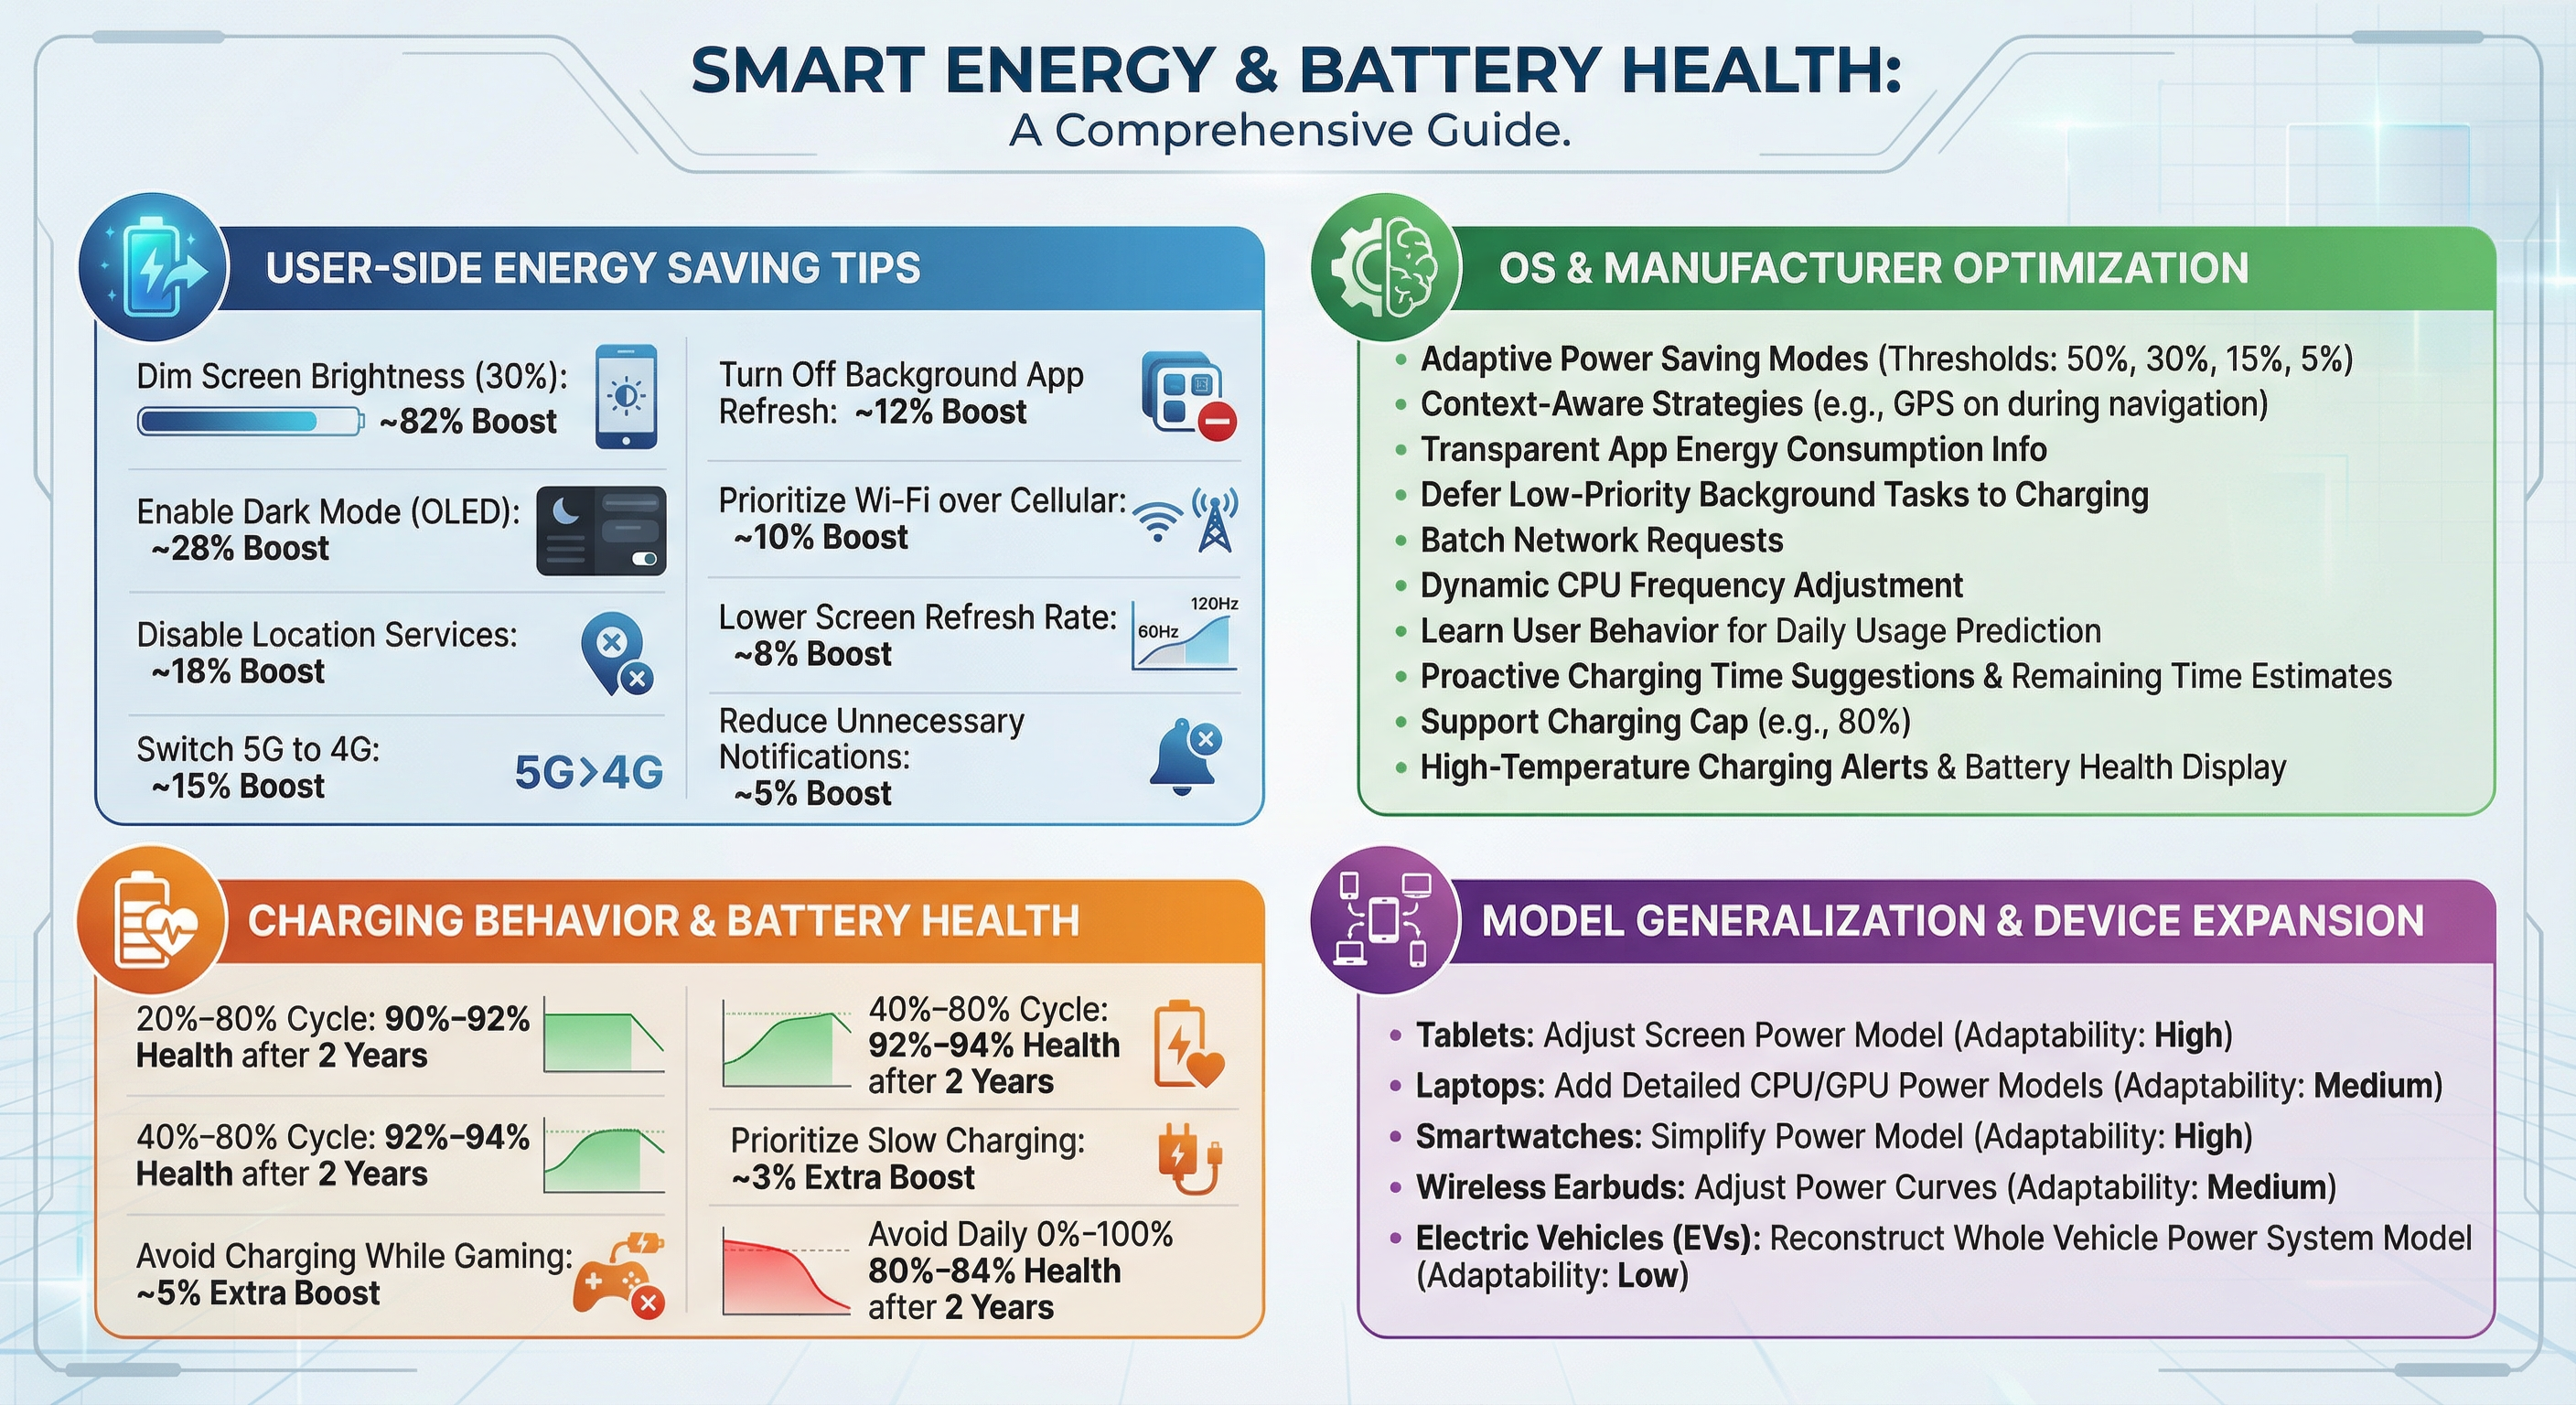
\includegraphics[width=0.85\textwidth]{figures/1770035421282-019c1e54-5bb0-7a65-98b2-ec7fd8e757ab.png}
    \caption{User recommendations overview.}
    \label{fig:user_recommendations}
\end{figure}

\subsection{Future Work}
\label{subsec:future}

Several extensions could enhance the model:

\begin{enumerate}
    \item \textbf{Machine Learning Enhancement:} Use neural networks to learn residual errors and improve predictions.
    
    \item \textbf{Distributed Thermal Model:} Implement 1D or 2D thermal models for better temperature prediction during high-power events.
    
    \item \textbf{Usage Pattern Learning:} Develop personalized models that learn individual user behavior patterns.
    
    \item \textbf{Cloud-Based Calibration:} Leverage fleet data to continuously improve parameter estimates.
    
    \item \textbf{Multi-Cell Extensions:} Extend the model to devices with multiple battery cells.
\end{enumerate}

